%%%%%%%%%%%%%%%%%%%%%%%%%%%%%%%%%%%%%%%%%%%
%%% DOCUMENT PREAMBLE %%%
%This template was adapted from a template by Roza Aceska.
\documentclass[12pt]{report}
\usepackage[english]{babel}
%\usepackage{natbib}
\usepackage{url}
\usepackage[utf8x]{inputenc}
\usepackage{amsmath}
\usepackage{graphicx}
\usepackage{parskip}
\usepackage{fancyhdr}
\usepackage{vmargin}
\setmarginsrb{3 cm}{2.5 cm}{3 cm}{2.5 cm}{1 cm}{1.5 cm}{1 cm}{1.5 cm}

\title{Report Assignment Part 1}								
% Title
\author{}						
% Author
\date{}
% Date

\makeatletter
\let\thetitle\@title
\let\theauthor\@author
\let\thedate\@date
\makeatother

\pagestyle{fancy}
\fancyhf{}
\rhead{\theauthor}
\lhead{\thetitle}
\cfoot{\thepage}
%%%%%%%%%%%%%%%%%%%%%%%%%%%%%%%%%%%%%%%%%%%%
\begin{document}

%%%%%%%%%%%%%%%%%%%%%%%%%%%%%%%%%%%%%%%%%%%%%%%%%%%%%%%%%%%%%%%%%%%%%%%%%%%%%%%%%%%%%%%%%

\begin{titlepage}
	\centering
    \vspace*{0.5 cm}
  \begin{center}    \textsc{\Large   Adavanced Process Mining SS20}\\[2.0 cm]	\end{center}
	\rule{\linewidth}{0.2 mm} \\[0.4 cm]
	{ \huge \bfseries \thetitle}\\
	\rule{\linewidth}{0.2 mm} \\[1.5 cm]
	
  \begin{minipage}{0.48\textwidth}
    \begin{flushleft} \large
      \emph{Submitted To:}\\
      Tobias Brockhoff\\
      Lisa Mannel\\
      Sebastiaan J. van Zelst MSc PhD\\
    \end{flushleft}
  \end{minipage}~
  \begin{minipage}{0.48\textwidth}
    \begin{flushright} \large
			\emph{Submitted By:} \\
      Student 1 (Matr. Number) \\
      Student 2 (Matr. Number) 
		\end{flushright}
	\end{minipage}\\[2 cm]
	
\end{titlepage}

%%%%%%%%%%%%%%%%%%%%%%%%%%%%%%%%%%%%%%%%%%%%%%%%%%%%%%%%%%%%%%%%%%%%%%%%%%%%%%%%%%%%%%%%%

\renewcommand{\thesection}{\arabic{section}}
General notes:
\begin{itemize}
  \item Remove this general note page and the text in \textlangle \textrangle
  \item This report should be at most 20 A4 pages, including the title page 
  \item	Data supporting your claims should be presented in a suitable and comprehensible aggregated form (diagrams, pictures, charts) and not as raw data tables (they can be added in the appendix)
  \item Submit this report as a PDF file
\end{itemize}
\newpage

\section{Q1. Inductive Miner}

As a first step into discovering the model for the event log, a short exploration was carried before the application of the algorithm. This to familiarize ourselves with the provided data. Besides a visualization of the dataset, a report was automatically generated with a data-centered description. Also, a brief analysis on the cardinality of the relation between traces and the \emph{Patient} column, which was found to be 1:1. Lastly, some random traces were visualized.

\paragraph{a)} 

Overall, we can estimate that the patients situation is assessed through an initial exam and, if necessary, 4 different treatments can be applied. In the process tree generated, visible in Figure \ref{fig:figures-q1_a_tree-pdf}, it is possible to identify the exclusive decision made between the discharge of the initial exam and the isolation inform, but the model fails to identify the relation between this decision and the application of the treatments, that certainly must occur only in infected patients.

\begin{figure}[h]
    \centering
    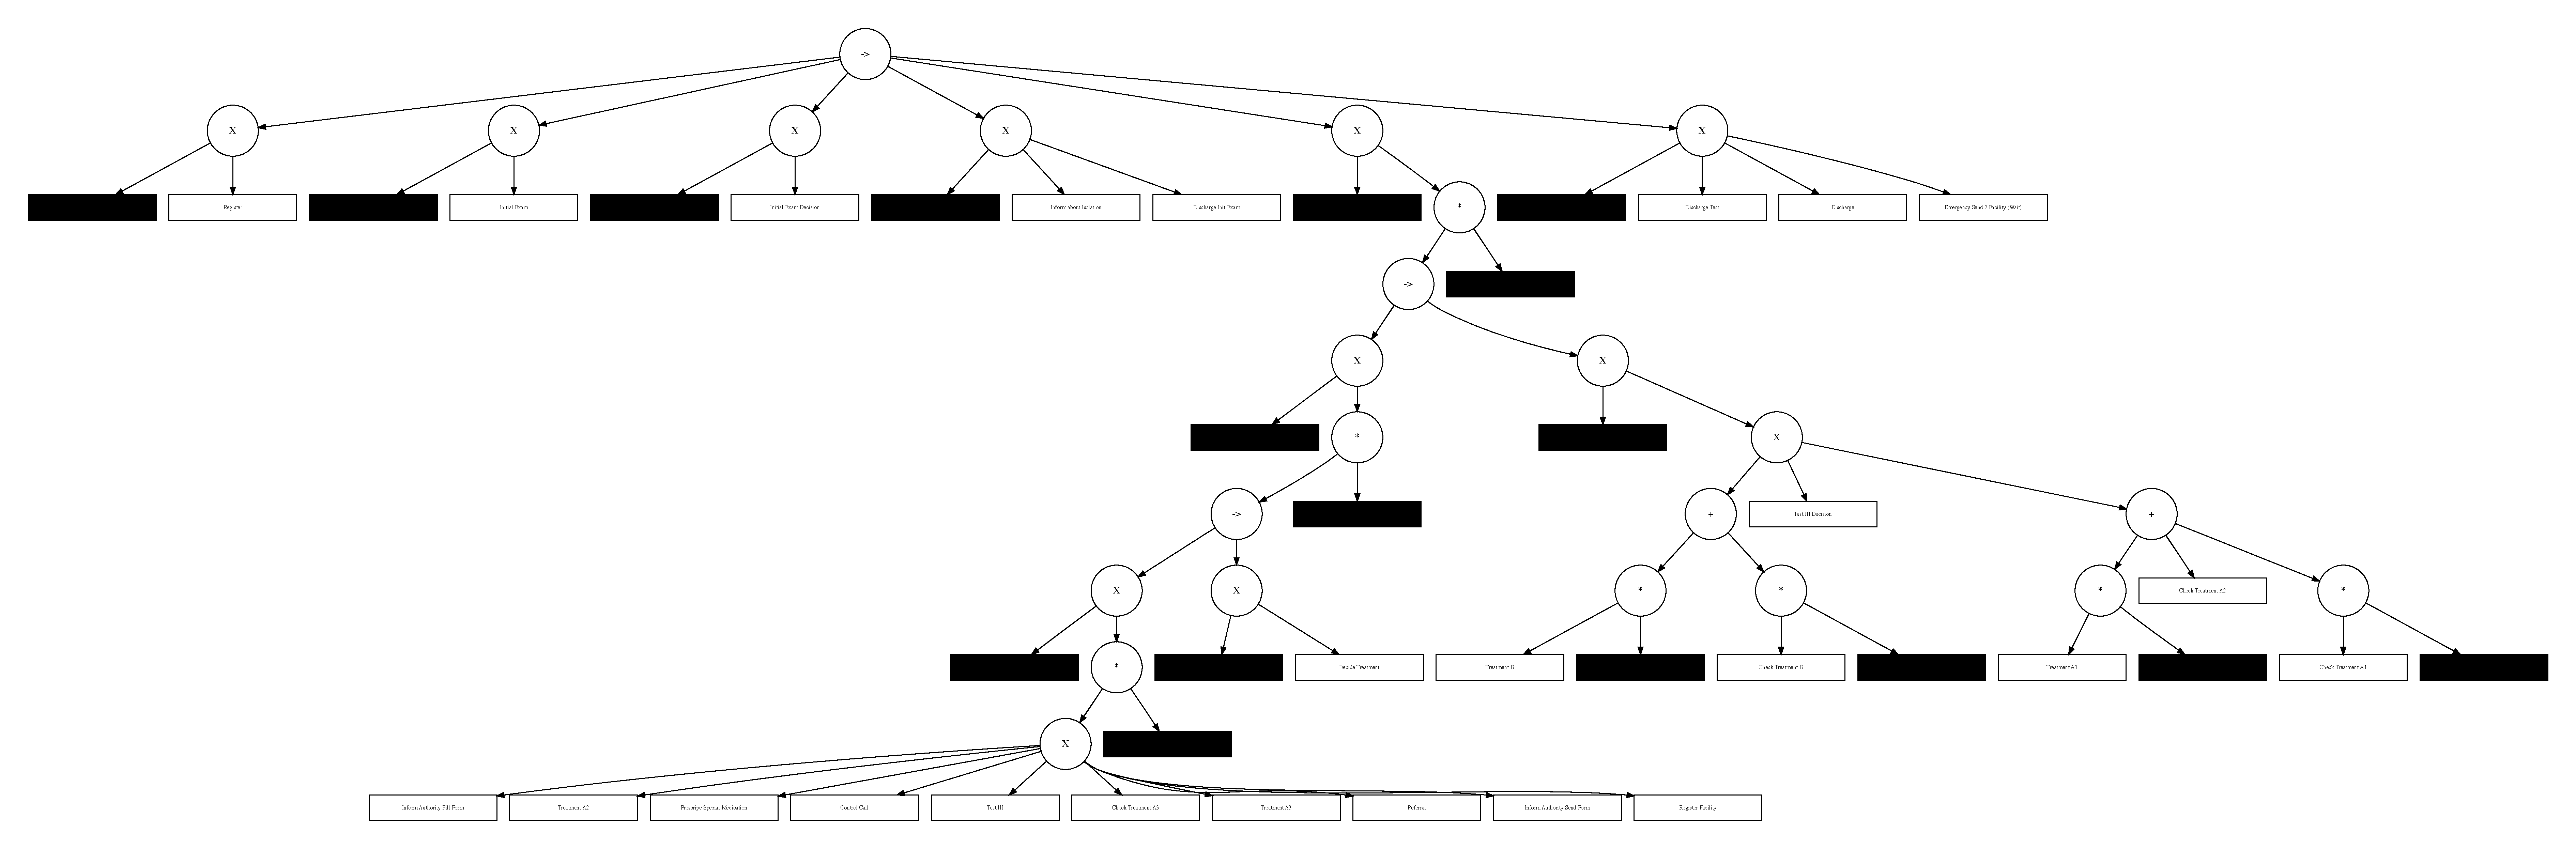
\includegraphics[width=0.8\textwidth]{figures/q1_a_tree.pdf}
    \caption{Process Tree generated by the Inductive Miner}
    \label{fig:figures-q1_a_tree-pdf}
\end{figure}

The treatments are applied multiple times alternating with the respective \emph{Check} activity. Unfortunately, the models are not too helpful in describing the choice of the treatments nor the dynamics of the execution of the remaining activities after the isolation inform. The exceptions are the ending activities, which tells us that the patients can either be discharged or sent to emergency care.

We notice the Inductive Miner guarantee for perfect fitness in the generated model through the presence of several silent transitions, an known outcome of the algorithm mainly present in the outcome of noisy event logs. Another characteristic of the IM is its inability to capture non-local dependencies, as it is shown more obviously, as already mentioned, by the lack of relation between the result of the initial exam and the applications' of the treatments. A more subtle consequence of this characteristic is the inability to constrain the `Check Treatment *` activities to follow, not necessarily directly, the respective treatment activity.

Regarding its precision, we notice there are several characteristics of the process that the model is unable to represent, using underfitting approaches instead. Besides the two mentioned just above, we point out the flower structure in the lowest level of the process tree and the more abstract flower pattern in the second-last exclusive choice operator of the second level. Therefore, we can say that the generated model is perfectly fit to the log, as expected, but not very precise.

The two main reasons identified for the lack of preciseness are the excess of silent transitions and the use of generalist structures (flower pattern). We can estimate that the first may be caused by noise in the data, which is usual. The second can be caused by a limitation of the algorithm, that is unable to deal with non-local dependencies.

\paragraph{b)} 

After distinguishing the two instances of the \emph{Control Call} activity in the event log, the Inductive Miner was again applied and the resulting model can be seen in Figure \ref{fig:figures-q1_b_tree-pdf} below.

\begin{figure}[h]
    \centering
    
\includegraphics[width=0.8\textwidth]{figures/q1_b_tree.pdf}
    \caption{Process Tree after \emph{Control Call} splitting}
    \label{fig:figures-q1_b_tree-pdf}
\end{figure}

We can see that not only the `Control Call` activity was removed from the flower structure at the bottom, but also the `Test III` and `Test III Decision` were brought up to the first sequence operator, of course still within a exclusive-choice operator with a silent activity, due to the noise on the data.

Still, now it is possible to extend our assumptions about the process. After the initial exam proceedings, several control calls can be performed and they are followed by the \emph{Test III}, which defines if the patient will need treatment.

\paragraph{c)} \textlangle Provide the answer here\textrangle
\paragraph{d)} \textlangle Provide the answer here\textrangle
\paragraph{e)} \textlangle Provide the answer here\textrangle
\paragraph{f)} \textlangle Provide the answer here\textrangle

\section{Q2. Social Network Analysis}
\textlangle Optional: Introduction \textrangle
\paragraph{a)} \textlangle Provide the answer here\textrangle
\paragraph{b)} \textlangle Provide the answer here\textrangle
\paragraph{c)} \textlangle Provide the answer here\textrangle
\paragraph{d)} \textlangle Provide the answer here\textrangle

\section{Q3. Performance Analysis}
\textlangle Optional: Introduction \textrangle
\paragraph{a)} \textlangle Provide the answer here\textrangle
\paragraph{b)} \textlangle Provide the answer here\textrangle

\section{Q4. Decision Points}
\textlangle Optional: Introduction \textrangle
\paragraph{a)} \textlangle Provide the answer here\textrangle
\paragraph{b)} \textlangle Provide the answer here\textrangle

\section{Q5. Proccess Improve Suggestions}
\textlangle Optional: Introduction \textrangle \\
\textlangle Provide the answer here\textrangle

\newpage
\section{Appendix}

\end{document}

